%%
%% sample document for AAMAS'19 conference
%%
%% modified from sample-sigconf.tex
%%
%% see ACM instructions acmguide.pdf
%%
%% AAMAS-specific questions? F.A.Oliehoek@tudelft.nl
%%

\documentclass[sigconf]{aamas}  % do not change this line!

%% your usepackages here, for example:
\usepackage{booktabs}
\usepackage{amsfonts, amsmath, amssymb, mathrsfs}
\usepackage{times, helvet, courier}
\usepackage{graphicx, epsfig, epstopdf}
\usepackage{wrapfig, caption, multirow, url}
\usepackage{mathptmx}
\usepackage{hyperref}
\usepackage{graphicx}
\usepackage{picinpar}
\usepackage{xcolor}
\usepackage{amsmath}
\usepackage{url}
\usepackage{csquotes}
\usepackage{listings}
\usepackage{algorithm}
\usepackage{algorithmic}
\usepackage{todonotes}

%% do not change the following lines
%\usepackage{flushend}
\setcopyright{ifaamas}  % do not change this line!
\acmDOI{doi}  % do not change this line!
\acmISBN{}  % do not change this line!
\acmConference[AAMAS'20]{Proc.\@ of the 19th International Conference on Autonomous Agents and Multiagent Systems (AAMAS 2020), B.~An, N.~Yorke-Smith, A.~El~Fallah~Seghrouchni, G.~Sukthankar (eds.)}{May 2020}{Auckland, New Zealand}  % do not change this line!
\acmYear{2020}  % do not change this line!
\copyrightyear{2020}  % do not change this line!
\acmPrice{}  % do not change this line!

%% the rest of your preamble here
\newcommand{\specialcell}[2][c]{%
	\begin{tabular}[#1]{@{}c@{}}#2\end{tabular}}
\renewcommand{\P}{{\mathcal P}}
\newcommand{\tbeg}{\langle}
\newcommand{\tend}{\rangle}
\newcommand{\entails}{\vDash}
\newcommand{\proves}{\vdash}
\newcommand{\union}{\cup}
\newcommand{\intersect}{\cap}
\newcommand{\compl}{\overline}
\newcommand{\lpnot}{\mbox{not}\;\,}
\newcommand{\lpor}{\;\,\mbox{\textsc{or}}\;\,}
\newcommand{\dlvif}{:\sim}
\newcommand{\sif}{\stackrel{\,\,\sim}{\leftarrow}}
\newcommand{\hif}{\leftarrow}
\newcommand{\dif}{\stackrel{\,\,-}{\leftarrow}}
\newcommand{\rif}{\stackrel{\,\,+}{\leftarrow}}
\newcommand{\impactsneg}{\ \mbox{impacts}_{\mbox{neg}}\ }
\newcommand{\impactspos}{\ \mbox{impacts}_{\mbox{pos}}\ }
\newcommand{\causes}{\mbox{ causes }}
\newcommand{\lawif}{\mbox{ if }}
\newcommand{\caused}{\mbox{ caused }}
\newcommand{\impossibleif}{\mbox{ impossible\_if }}
\newcommand{\triggers}{\mbox{ triggers }}
\newcommand{\defaults}{{\mathsf{defaults}}}%{\mbox{ defaults }}

\makeatletter
\DeclareRobustCommand*\cal{\@fontswitch\relax\mathcal}
%\def\@textbottom{\vskip \z@ \@plus 1pt}
%\let\@texttop\relax
\makeatother

\usepackage{listings}
\lstdefinelanguage{clingo}{
  keywordstyle=[1]\usefont{OT1}{cmtt}{m}{n},%
  keywordstyle=[2]\textbf,%
  keywordstyle=[3]\usefont{OT1}{cmtt}{m}{n},%\textit
  alsoletter={\#,\&},%
  keywords=[1]{not,from,import,exists,if,else,return,while,
  break,and,or,for,in,del,and,class,subClass,relevantToFunc,
  concern,aspect,subconcern,property,rdf,cpsf,addressedBy,component,higher_TW,componentHoldProperty,count_addresses,count_relations,truthworthiness_comp,highest_TW,input,addrForConcern,relation,holds,obs},%
  keywords=[2]{\#const,\#show,\#minimize,\#base,\#theory,\#count,\#external,\#program,\#script,\#end,\#heuristic,\#edge,\#project,\#show,\#sum},%
  keywords=[3]{&,&dom,&sum,&diff,&show,&minimize},%
  morecomment=[l]{\#\ },%
  morecomment=[l]{\%\ },%
  commentstyle={\color{darkgray}}%
}
\lstset{numbers=left,numberblanklines=false,basicstyle=\ttfamily\small,language=clingo}
\lstset{escapeinside={*@}{@*}}

%%%%%%%%%%%%%%%%%%%%%%%%%%%%%%%%%%%%%%%%%%%%%%%%%%%%%%%%%%%%%%%%%%%%%%%%%%%%%%%%%%%%%%%%%%%%%%%%%%%%%%%%%

\begin{document}

\title{Cyber-Physical System}  % put your title here!
%\titlenote{Produces the permission block, and copyright information}

% AAMAS: as appropriate, uncomment one subtitle line; check the CFP
%\subtitle{Extended Abstract}
%\subtitle{Blue Sky Ideas Track}
%\subtitle{JAAMAS Track}
%\subtitle{Demonstration}
%\subtitle{Doctoral Consortium}

% AAMAS: submissions are anonymous for most tracks
\author{Paper \#XXX}  % put your paper number here!

%% example of author block for camera ready version of accepted papers: don't use for anonymous submissions
%
%\author{Ben Trovato}
%\authornote{Dr.~Trovato insisted his name be first.}
%\orcid{1234-5678-9012}
%\affiliation{%
%  \institution{Institute for Clarity in Documentation}
%  \streetaddress{P.O. Box 1212}
%  \city{Dublin} 
%  \state{Ohio} 
%  \postcode{43017-6221}
%}
%\email{trovato@corporation.com}
%
%\author{G.K.M. Tobin}
%\authornote{The secretary disavows any knowledge of this author's actions.}
%\affiliation{%
%  \institution{Institute for Clarity in Documentation}
%  \streetaddress{P.O. Box 1212}
%  \city{Dublin} 
%  \state{Ohio} 
%  \postcode{43017-6221}
%}
%\email{webmaster@marysville-ohio.com}
%
%\author{Lars Th{\o}rv{\"a}ld}
%\authornote{This author is the
%  one who did all the really hard work.}
%\affiliation{%
%  \institution{The Th{\o}rv{\"a}ld Group}
%  \streetaddress{1 Th{\o}rv{\"a}ld Circle}
%  \city{Hekla} 
%  \country{Iceland}}
%\email{larst@affiliation.org}
%
%\author{Valerie B\'eranger}
%\affiliation{%
%  \institution{Inria Paris-Rocquencourt}
%  \city{Rocquencourt}
%  \country{France}
%}
%\author{Aparna Patel} 
%\affiliation{%
% \institution{Rajiv Gandhi University}
% \streetaddress{Rono-Hills}
% \city{Doimukh} 
% \state{Arunachal Pradesh}
% \country{India}}
%\author{Huifen Chan}
%\affiliation{%
%  \institution{Tsinghua University}
%  \streetaddress{30 Shuangqing Rd}
%  \city{Haidian Qu} 
%  \state{Beijing Shi}
%  \country{China}
%}
%
%\author{Charles Palmer}
%\affiliation{%
%  \institution{Palmer Research Laboratories}
%  \streetaddress{8600 Datapoint Drive}
%  \city{San Antonio}
%  \state{Texas} 
%  \postcode{78229}}
%\email{cpalmer@prl.com}
%
%\author{John Smith}
%\affiliation{\institution{The Th{\o}rv{\"a}ld Group}}
%\email{jsmith@affiliation.org}
%
%\author{Julius P.~Kumquat}
%\affiliation{\institution{The Kumquat Consortium}}
%\email{jpkumquat@consortium.net}
%
%% The example's default list of authors is too long for headers
%\renewcommand{\shortauthors}{B. Trovato et al.}


\begin{abstract}  % put your abstract here!

\end{abstract}


\keywords{CPS; Action and Changes; ASP}  % put your semicolon-separated keywords here!

\maketitle

%%%%%%%%%%%%%%%%%%%%%%%%%%%%%%%%%%%%%%%%%%%%%%%%%%%%%%%%%%%%%%%%%%%%%%%%%%%%%%%%%%%%%%%%%%%%%%%%%%%%%%%%%
%% start of main body of paper

\section{Introduction}

\begin{list}{$\bullet$}{\itemsep=0pt \parsep=1pt \topsep=1pt \leftmargin=12pt} 
\item Cyber-physical systems (CPS) combine cyber capabilities (computation and/or communication) with physical capabilities (motion or other physical processes).
 
\item Cars, aircraft,
and robots are prime examples, because they move physically in space in a way that is determined by discrete computerized control algorithms

\item CPS framework provides the taxonomy and methodology for designing, building, and assuring cyber-physical systems that meet the expectations and concerns of system stakeholders.

\item Ontology reasoning: Answer Set Programming
\end{list}



\section{Background}
%
\subsection{A CPS Framework Ontology}
\label{sub-section:CPS_ontology}
%
At the core of this approach is an ontology of the CPS Framework and of a CPS of interest. An ontology is a formal, logic-based representation that supports reasoning by means of logical inference. In this paper, we adopt a rather broad view of this term: by ontology, we mean a collection of statements in a logical language that represent a given domain in terms of \emph{classes} (i.e., sets) of objects, \emph{individuals} (i.e., specific objects), relationships between objects and/or classes, and logical statements over these relationships.
In the context of the trustworthiness of CPS, for instance, an ontology might define the high-level concept of ``Concern'' with its refinement of ``Aspect.'' All of these will be formalized as classes and, for Aspect, subclasses. Specific concerns will be represented as individuals: $T\!rustworthiness$ as an individual of class Aspect, $Security$ and $Cybersecurity$ of class Concern.
Additionally, a relation ``has-subconcern'' might be used to associate a concern with its sub-concerns. Thus, Aspect ``has-subconcern'' $Security$, which in turn ``has-subconcern'' $Cybersecurity$. By introducing a property ``satisfied,'' one could also indicate which concerns are satisfied. 
%
Inference can then be applied to propagate ``satisfied'' and other relevant properties and relations throughout the ontology. For example, given a concern that is not ``satisfied,'' one can leverage relation ``has-subconcern'' to identify the concerns that are not satisfied, either directly or indirectly, because of it. 
%
In practice, it is often convenient to distinguish between the factual part, $\Omega$, of the ontology (later, simply called ``ontology''), which encodes the factual information (e.g., $T\!rustworthiness$ ``has-subconcern'' $Security$), and the \emph{axioms}, $\Lambda$, expressing deeper, often causal, links between relations (e.g., a concern is not satisfied if any of its sub-concerns is not satisfied). Further, when discussing reasoning tasks, we will also indicate, separately, the set $\mathcal{Q}$ of axioms encoding a specific reasoning task or query.
%
\subsection{Reasoning with Ontology and Answer Set Program}
\label{sub-section:asp_reasoning_ontology}
By leveraging a logic-based representation of a domain of interest, one can apply inference and draw new and useful conclusions in a principled, rigorous way. In essence,  our approach is agnostic to any specific choice of logical language and inference mechanisms. Axioms expressed in the used logical language formalize the queries one is interested in answering, the type of reasoning that can be carried out, and any additional contextual information.
Thus, given an ontology $\Omega$, a set of axioms $\Lambda$, and an inference relation $\entails$, we say that $\Delta$ is an answer to the (implicit) query iff
%
\[
\Omega \cup \Lambda \entails \Delta.
\]
where $\cup$ denotes the union of two sets. For instance, in the language of propositional logic, given knowledge that some proposition $p$ is true and that $p$ implies some other proposition $q$, one can infer that $q$ is also true, i.e.:
\[
\{p, p \supset q\} \entails \{q\}.
\]
In the context of cybersecurity, $p$ might be true when a cyberattack has occurred and $p \supset q$ might formalize an expert's knowledge that, whenever that cyberattack occurs, a certain system becomes inoperative (proposition $q$). The logical inference represented by symbol $\entails$ allows to draw the conclusion that, as a result of the cyberattack, the system is now inoperative. For increased flexibility of representation, we use here a non-monotonic extension of propositional logic, called Answer Set Programming (ASP)  \cite{SonP06b,SonBTM05}.

An ASP program is built on a signature consisting of a set of constants $\cal C$,
a set of variables $\cal X$ and a set of predicate symbols $\cal P$. The definitions
of terms and atomic formulae (atoms) are the traditional ones. An answer set program is a set of rules of the form: \\
\texttt{ $a_0 {:-} a_1, . . . , a_m$, not $ a_{m+1}, . . . ,$ not  $a_n$}, where 0 $\leq$ m $\leq$ n, each $a_i$ is an atom, and \texttt{not} represents \textit{negation-as-failure (naf)}. A naf-literal has the form \texttt{not $a$}, where $a$ is an atom. Given a rule of this form, the left and right hand sides are called the \textit{head} and \textit{body}, respectively. A rule may have either an empty head or empty body, but not both. Rules with an empty head are called \textit{constraints}---the empty head is implicitly assumed to represent \texttt{False}; rules with an empty body are known as \textit{facts}. The language allows the use of variables, and they are simply viewed as placeholders for any element of $\cal C$; thus a rule with variables (non-ground) is simply a syntactic sugar for the set of rules obtained by consistently replacing each variable with any element of $\cal C$ (ground rules).

A set of ground atoms $X$ satisfies the body of a ground rule if \{$a_{m+1}, . . . , a_n$\} $\cap$ \texttt{X} = $\emptyset$ and \{$a_1, . . . , a_m$\} $\subseteq$ $X$. A \textit{constraint} is \textit{satisfied} by $X$ if its body is not satisfied by $X$. $X$ is a model of a rule if either it does not satisfy the body or $a_0 \in X$. $X$ is a model of a program if it satisfies all of its rules.

 If a ground program $\Pi$ does not contain any naf-literals, then the semantics of $\Pi$ is given by its unique subset-minimal model.
Given a ground program $\Pi$ and a set of ground atoms $X$, the \textit{reduct} of \texttt{$\Pi$} w.r.t \texttt{X} (denoted by \texttt{$\Pi^X$}) is the program obtained from  \texttt{$\Pi$} by: ({\em i}) deleting all the rules that have a naf-literal \texttt{not} $a$ in the body and $a$ $\in$ $X$, and ({\em ii}) removing all
remaining naf-literals.

A set of ground atoms $X$ is an \textit{answer set} of a program {$\Pi$} if $X$ is the subset-minimal model of $\Pi^X$.
Several syntactic extensions have been introduced to facilitate the development of program. For example, \emph{choice atoms}
have the form $l\:\{b_1, . . . , b_k\}\:u$, where each $b_j$ is an atom, and $l$ and $u$ are integers such that $l$ $\leq$ $u$.
 A set of atoms $X$ satisfies a choice atom $l$\{$b_1, . . . , b_k$\}$u$ if $l$ $\leq$ $|X$  $\cap $ \{$b_1, . . . , b_k$\}$| \leq u$.
 Non-ground versions of choice atoms allow the use of syntax analogous to that of intensional sets, e.g., $l\:\{p$($X$)$:q$($X$)$\}\:u$.
%
\subsection{Representing Ontology in ASP}
\label{sub-section:asp_representation}
%
The entities of the CPS Ontology (classes, instances and properties) are represented in ASP using unary predicate {\tt \small class} and the binary predicate {\tt \small subClass}. The predicate {\tt \small class(X)}, {\tt \small subClass(X,Y)} say that {\tt \small X} is a class, {\tt \small X} is a subclass of {\tt \small Y}, respectively. To reason about subclass relationship, the encoding contains the rule {\tt \small subClass(X,Y) :- subClass(Z,Y), subClass(X,Z).}

The predicate {\tt \small aspect(I)}, {\tt \small concern(I)}, {\tt \small property(I)} denotes that {\tt \small I} is an individual of class aspect, concern and property, respectively. For example, in CPS ontology, \emph{concern}, \emph{aspect} and \emph{property} are classes and \emph{aspect} is subclass of \emph{concern}. There are nine aspects (highest level concerns) (e.g., \emph{trustWorthiness}, \emph{business}, \emph{timing}, etc.) and they are individuals of class \emph{aspect}. In addition, there are many instances of class \emph{concern} such as: \emph{security}, \emph{reliability}, \emph{functionality}, \emph{cyber-security}, \emph{physical-security} etc. In which, \emph{cyber-security} and \emph{physical-security} are sub-concerns of \emph{security}. Concern \emph{security}, \emph{reliability} are sub-concerns of \emph{trustWorthiness}. The predicate {\tt \small subconcern(I,J)} denotes that concern {\tt \small J} is sub-concern of concern {\tt \small I}. All above entities and their relations are described in ASP by the set of facts:
\begin{lstlisting}[language=clingo,caption=ASP representation aspects and concerns in Ontology $\Omega$, label=list4, mathescape=true,xleftmargin=.01\textwidth, breaklines=true]
class(concern). class(aspect). class(property).
subClass(aspect,concern).
aspect(trustWorthiness). aspect(business). aspect(timing). 
concern(security). concern(reliability). concern(functionality). 
concern(cyber-security). concern(physical-security).
subconcern(trustWorthiness,security). subconcern(trustWorthiness,reliability).
subconcern(security,cyber-security). subconcern(security,physical-security).
\end{lstlisting}
In the current system, the CPS Ontology is queried by {\tt SparQL} language to retrieve all RDF triplestores. Each RDF triplestore is a tuple {\tt (S,P,O)} ({\tt S}: Subject, {\tt P}: Predicate or Verb, {\tt O}:Object) that is encoded in ASP by atom of the form {\tt input(S,P,O)}.

\begin{lstlisting}[language=clingo,caption=ASP reasoning RDF triplestores in Ontology $\Omega$, label=lst:RDF_triplestore_ecoding, mathescape=true,xleftmargin=.01\textwidth, breaklines=true]
property(P):-input(P,"rdf:type","cpsf:Property").
concern(C) :- input(C,"rdf:type","cpsf:Concern").
aspect(A) :- input(A,"rdf:type","cpsf:Aspect").
subconcern(S,O):- input(S,"cpsf:includesConcern",O).
% Aspect is a concern and is subconcern of "all"
concern(A) :- aspect(A).
concern(all).
subconcern(all,A) :- aspect(A).
relevantToFunc(C,F) :- input(C,"cpsf:relevantToFunc",F).
relevantToFunc(C1,F) :- relevantToFunc(C2,F), subconcern(C1,C2).
\end{lstlisting}
%
Properties of CPS are represented by individual of class {\tt Property}. The relation between concern $C$ and property $P$ is represented by the predicate {\tt \small addressedBy(C,P)} which denotes that concern $C$ is address by property $P$.
\begin{lstlisting}[language=clingo,caption=The relation between Properties and Concerns in $\Omega$, label=lst:address_encoding, mathescape=true,xleftmargin=.01\textwidth, breaklines=true]
addressedBy(C,P):- concern(C), property(P), input(C,"cpsf:addressedByProperty",P), ).
addressedBy(C,P):-addressedBy(C1,P), subconcern(C,C1).
\end{lstlisting}
%  
In ASP representation, each \emph{configuration} (e.g, in listing~\ref{lst:configuration_ecoding}) includes a set of facts in the ASP form {\tt obs(conf,true)} which denote that in the initial state of CPS system, the fluent {\tt conf} holds at step 0 (Line 1-7). Line 8 denotes that a property $X$ was impacted negatively then it does not hold. 
In CPS ontology, the terminology \emph{Configuration} presents the current state of CPS system and each individual of class \emph{Configuration} represents a different configuration feature.
\begin{lstlisting}[language=clingo,caption=ASP reasoning Configurations (Initial State) in $\Omega$, label=lst:configuration_ecoding, mathescape=true,xleftmargin=.01\textwidth, breaklines=true]
obs(sat("encrypted_mem_input1"),true).
obs(sat("encrypted_mem_sam"),true).
obs(sat("sec_boot_input1"),true).
obs(sat("sec_boot_sam"),true).
obs(sat("slow_mode_input1"),true).
holds(F,0) :- fluent(F), obs(F,true).
-holds(F,0) :- fluent(F), obs(F,false).
-holds(X,T) :- impacted(neg,X,T).
\end{lstlisting}

\begin{lstlisting}[language=clingo,caption=An example of negative impaction of a property, label=lst:example_neg_impact, mathescape=true,xleftmargin=.01\textwidth, breaklines=true]
impacted(neg,sat("consist_reading_freq_input1"),S) :- step(S), holds(sat("using_basic_input1"),S),holds(sat("encrypted_mem_input1"),S), -holds(sat("slow_mode_input1"),S).
\end{lstlisting}
%
\textbf{Constraints, dependencies, trade-offs.} An additional feature of our model is the ability to establish causal links between concerns, properties, configurations,  and actions. This is accomplished by the reasoning over statements. Table~\ref{tab:constraints} lists types of statements, their syntactic expressions as judgments, and their corresponding encodings for the ASP reasoner. The logical encodings of the statements are used to implement reasoning capabilities discussed later in the paper. $\Gamma$ and $\pi$ range over (sets of) propositions and $a$ over actions.
\begin{table}[htbp]
	\begin{small}
		\begin{center}
			\begin{tabular}{|l|l|l|}
				\hline
				\textbf{Statement type} & \textbf{Syntax} & \textbf{Encoding for reasoner} \\
				\hline
				\specialcell[c]{\hspace*{-.2in}$\mbox{Property}$\\$\mbox{dependency}$} & 
				\specialcell[c]{$\Gamma \impactspos \pi$ \\
					$\Gamma \impactsneg \pi$} &
				\specialcell[c]{\!\!$impacted$($pos$/$neg,\pi,S$)$ \hif$ \\$holds$($\Gamma,S$)}\\
				\hline
				\specialcell[c]{$\mbox{Default property}$\\$\mbox{\hspace*{-.56in}value}$}
				& 
				\specialcell[c]{$\sigma\ \defaults\ true$ \\
					$\sigma\ \defaults\ f\!alse$} &
				\!\!$\defaults$($\sigma,true/false$)\\
				\hline
				Effects of actions & $a \causes \pi \lawif \Gamma$ &
				\specialcell[c]{\hspace*{-.4in}$holds$($\pi,S+1$)$ \hif$ \\$\ \ holds$($\Gamma,S$)$, occurs$($a,S$)}\\
				\hline
				Triggered actions & $\Gamma \triggers a$ &
				\!\!$occurs$($a,S$)$ \hif holds$($\Gamma,S$)\\
				\hline
			\end{tabular}
		\end{center}
	\end{small}
\vspace*{-.01in}  % correct bad spacing due to \setlength{\belowcaptionskip}
\caption{Constraints, dependencies, and trade-offs where $\Gamma$, $\pi$ range over (sets of) propositions and $a$ over actions}\label{tab:constraints}
\end{table}
%
For example of a property dependency statement, Rule 1 in listing~\ref{lst:example_neg_impact} encodes that when the basic type of device {\tt input1} is in use and {\tt input1} is using encrypted memory and fast mode impacts negatively the maintainability of a consistent reading frequency. %Line 2 states that if property $X$ was impacted negatively then it does not hold.
%
\subsection{A Use Case}
\label{sub-section:use_case}
%
For sake of illustration, in a lane keeping/assist (LKAS) use case centered around an advanced car that uses a camera ({\tt CAM}) and a situational awareness module ({\tt SAM}). The SAM processes the video stream from the camera and controls, through a physical output, the automated navigation system. The camera and the SAM may use encrypted memory and secure boot. Safety mechanisms in the navigation system cause it to shut down if issues are detected in the input received from the SAM. This use case is chosen because it encompasses major component types of a CPS, and lends itself to various non-trivial investigations. Through this use case, we will highlight the interplay among trustworthiness concerns, as well as their ramifications on other CPS aspects, such as the functional aspect.
%

Assuming that the camera is capable of two recording modes, one at 25 fps (frames per second) and the other at 50 fps. The selection of the recording mode is made by SAM, by acting on a flag of the camera's configuration. It is assumed that two camera models exist, a basic one and an advanced one. Either type of camera can be used when realizing the CPS. Due to assumed technical limitations, the basic camera is likely to drop frames if it attempts to record at 50 fps while using encrypted memory.
%

The decomposition of a CPS identifies resources that may satisfy properties. Suppose that {\tt CAM} is a camera, a subsystem of an autonomous car, and that {\tt SAM} is a memory sub-system of {\tt CAM}; we will examine this system in more detail later. Then {\tt cam\_mem[encr]}, e.g., is a Boolean predicate that is true if the memory {\tt mem} of camera {\tt CAM} uses encryption. Properties thus have form {\tt SystemPath[prop]} where {\tt SystemPath} identifies a system component or part, with sub-components indicated by the underscore symbol, and {\tt prop} a property that this part may enjoy. 
%We interpret two such properties to be equal only if their actual names are equal: {\tt cam\_mem1[encr]} and {\tt cam\_mem2[encr]}, e.g., are different properties as the same encryption is applied to different memories of the same camera {\tt CAM}.
Properties {\tt SystemPath[prop]} also have a semantic context {\tt ConcernPath} that articulates which (sub)concern of an aspect this property is trying to address.
In our semantics below, a property may be either true or false (i.e., satisfied or non-satisfied). These truth values in turn influence the satisfaction of concerns and aspects.
%

\section{Formalization}


\subsection{Formalization CPS ontology}
\label{for:CPS_ontology}
The formalization of a CPS is organized along multiple levels: (L1) aspects and concerns; (L2) properties; (L3) CPS configuration; (L4) actions; (L5) constraints, dependencies and trade-offs; and (L6) satisfaction axioms. Level L1 and L6 form the \emph{CPS-independent specification}, since aspects and concerns are independent of the specific CPS being modeled. Levels L2-L5 comprise the \emph{CPS-dependent specification}, as the information included in them depends on the CPS being modeled. Furthermore, levels L1 and L2 formalize the concepts from the definition of the CPS Framework. Levels L3-L5 extend the CPS Framework in order to provide details needed for reasoning about the behavior of a CPS of interest. Level L6 provides the semantics of the formalization. The ASP representation for 6 levels of CPS ontology is described in section ~\ref{sub-section:asp_representation}

\subsection{A Physical CPS System}
\label{for:physical_CPS_system}
\begin{definition}
\label{def:physical_CPS_system} 
A physical CPS system $S$ is a tuple ($C, A, F, R$) where:
%
\begin{list}{$\bullet$}{\itemsep=0pt \parsep=1pt \topsep=1pt \leftmargin=12pt} 
\item $C$ is a set of physical components.
\item $A$ is a finite set of actions that can be execute over CPS system.
\item $F$ is a finite set of fluent literals.
\item $R$ is a set of relations that map each physical component $c \in C$ with a set of physical component properties that are defined in CPS Ontology.  \\
For any $r \in R$, $r : C \longrightarrow 2^{P_{C}}$. In which, we have $2^{P_{C}}$ is power set of $P_{C}$, $P_{C}$ is set of properties which related to physical components, $P$ is set of all properties that are defined in CPS ontology ~\ref{sub-section:CPS_ontology} and $P_{C} \subset P$. 
\end{list}
%
\end{definition}
%
Intuitively, the CPS problem related the example in use case ~\ref{sub-section:use_case} can be specified by $S_{auto} = $ ($C_{auto}, A_{auto}, F_{auto}, R_{auto}$) where:
\begin{list}{$\bullet$}{\itemsep=0pt \parsep=1pt \topsep=1pt \leftmargin=12pt} 
\item $C_{auto} = \{{\tt SAM}, {\tt CAM}\}$ .
\item $A_{auto}$ is set of finite actions which consists of:
\begin{list}{$\bullet$}{\itemsep=0pt \parsep=1pt \topsep=1pt \leftmargin=12pt} 
\item {\tt \small switMem(X,encrypted),switMem(X,unencrypted)}: denote actions to switch component $X$ using encrypted or unencrypted memory respectively. 
\item {\tt \small switReMod(X,50fps),switReMod(X,25fps)}: denote actions to switch component $X$ using 50 fps and 25 fps recording modes respectively. 
\item {\tt \small switModel(X,basic),switReMod(X,advanced)}: denote actions to switch component $X$ using basic and advanced models respectively. 
\item etc. (should be more)
\end{list}
\item $F_{auto}$ is a finite set of fluent literals which consists of:
\begin{list}{$\bullet$}{\itemsep=0pt \parsep=1pt \topsep=1pt \leftmargin=12pt} 
\item {\tt \small useMem(X,encrypted),useMem(X,unencrypted)}: denote that component $X$ is using encrypted or unencrypted memory respectively. 
\item {\tt \small recordMode(X,50fps),recordMode(X,25fps)}: denote that component $X$ is recording video with 50 fps and 25 fps modes respectively. 
\item {\tt \small useModel(X,basic),useModel(X,advanced)}: denote that component $X$ is working on basic and advanced models respectively. 
\item etc. (should be more)
\end{list}
\item $R_{auto} =\{${\tt CAM} $\mapsto \{{\tt reMode\_50fps, model\_basic,...}\}$, {\tt SAM} $\mapsto \{{\tt mem\_encrypted, boot\_sec,...}\}$  $\}$ \\
In which, {\tt \small reMode\_50fps, reMode\_25fps, model\_basic, mem\_encrypted, boot\_sec, etc.}  are defined in CPS Ontology properties ~\ref{sub-section:CPS_ontology}. 
\end{list}
\subsection{Truthworthiness Problem Definition}
\emph{Truthworthiness} is one of nine highest level concerns (\emph{aspects}) and a critical concern stakeholders have about CPS and the Internet of Things (IoT) and their development.There, \emph{trustworthiness} is captured as a high-level concern encompassing safety, security, privacy, resilience, and reliability. While there are many efforts, in multiple sectors, to study these characteristics of systems they are typically considered separately and in isolation. This can result in work, intended to address one of these concerns, adversely impacting work to address one or more of the others. Thus CPS/IoT trustworthiness relies on an integrated, concern-driven approach that takes into account the interactions between the cyber and physical elements of systems. There are some important \emph{Truthworthiness} queries which should be answered in CPS system: 
\begin{itemize}
	\item Is the Truthworthiness aspect satisfied? 
	\item What is the most vulnerability in CPS system?
	\item If there exists the vulnerability in CPS system, how to fix it?
\end{itemize}
\begin{figure}
	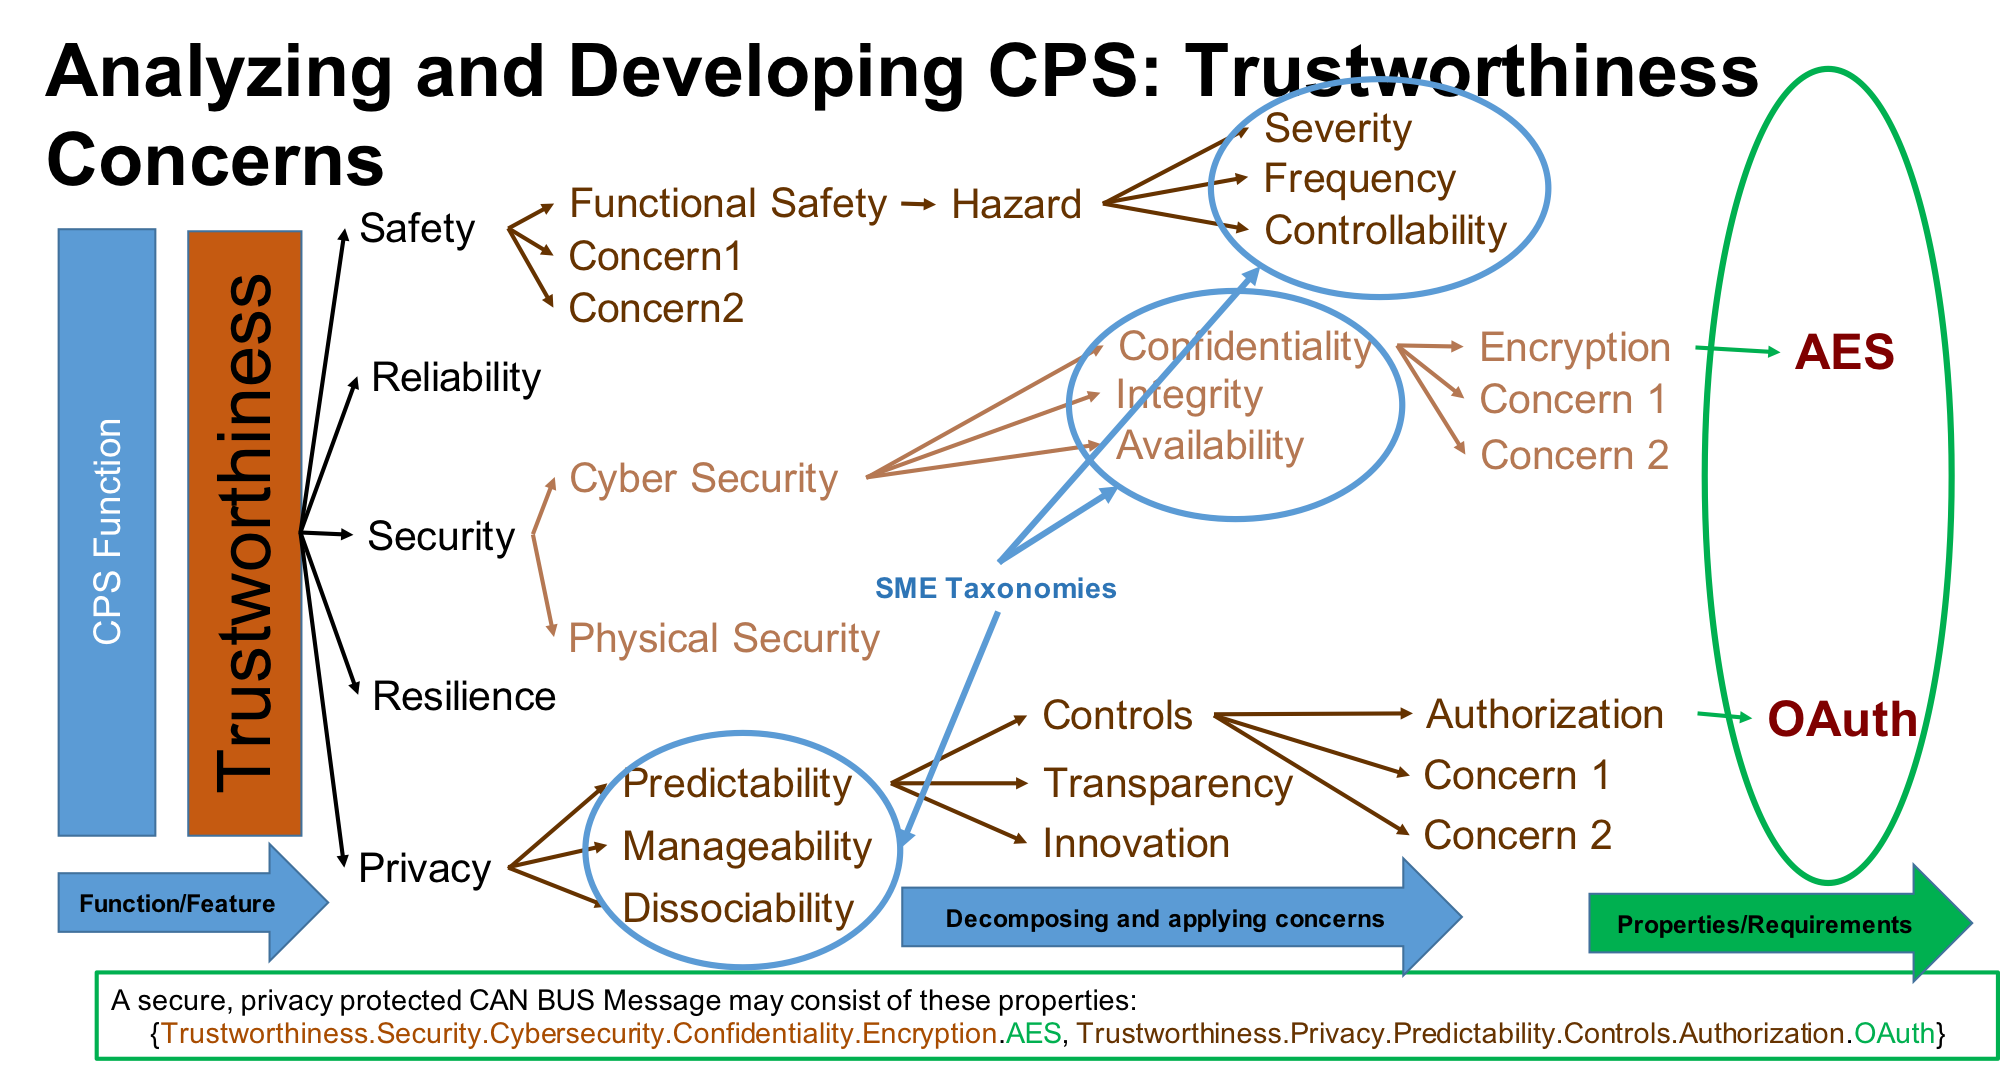
\includegraphics[width=250pt]{trustconcerntree.png}
	\caption{Decomposition tree for Trustworthiness Concerns\label{fig:trustworthiness}}
\end{figure}

\subsection{Probability of success of mitigation strategies}
\begin{definition}
	\label{def:probability_of_success} 
	
\end{definition}

\subsection{Likelihood of Concerns Satisfaction}
\begin{definition}
	\label{def:likelihood_concern_sat} 
	
\end{definition}

\subsection{Vulnerability in CPS System}
\begin{definition}
	\label{def:vulnerability} 
	
\end{definition}

\begin{proposition}
	\label{pro:most_vulnerability} 
	
\end{proposition}

\section{Implementation}
%
\subsection{Query 1: Is the Truthworthiness aspect satisfied?}
%
\begin{lstlisting}[language=clingo,caption=Reasoning for the satsifaction of aspect, label=lst:q_1_reasoning_satisfaction, mathescape=true,xleftmargin=.01\textwidth, breaklines=true]
-holds(sat(C),T):-addressedBy(C,$\pi$),not holds($\pi$,T).
-holds(sat(C),T) :-addressedBy(C,$\pi$),-holds($\pi$,T).
-holds(sat($C_1$),T) :-subconcern($C_1$,$C_2$),not holds(sat($C_2$),T).
-holds(sat($C_1$),T) :-subconcern($C_1$,$C_2$),-holds(sat($C_2$),T).
holds(X,T) :- defaults(X,true), not -holds(X,T).
\end{lstlisting}
In this listing, $T$ denotes a discrete step in the evolution of the CPS. The inclusion of a step argument makes it possible to analyze the evolution of CPS over time in response to possible events. Lines 1-2 states that a concern $C$ is not satisfied if any of the properties that address it does not hold. This ensures that the lack of satisfaction of a property $\pi$ is propagated to the concern(s) that are addressed by $\pi$ according to the {\tt addressedBy/2} statements. Line 3-4 encodes that the lack of the satisfaction is then propagated up the concern tree according to the concern-concern relation specified by the {\tt subconcern/2} statements. The specification of the notion of satisfaction is completed by {\tt defaults} statements saying that all properties and concerns are satisfied by default (Line 5), which embodies the semantics of the {\tt defaults} statement in Table~\ref{tab:constraints}.
%

The probabilistic component was added to the model, supporting calculation of ({\bf 1}) \emph{probability of success of mitigation strategies} and ({\bf 2}) \emph{likelihood that concerns are satisfied} .

In probability of success of mitigation strategies, the fluent {\tt \small prob\_ of\_state(prob)} models the propagation by the model to the successor state and the statement {\tt holds(prob\_of\_state(prob) ,S)} means that  at step $S$ of the evolution the system, the probability in the current state described by the fluent is {\tt prob}. The statement {\tt do(a,S)} denotes that an action $a$ is executed at step $S$ of CPS evolution. The fluent {\tt prob\_success(a,$prob_a$)} denotes that an action $a$ has probability $prob_a$ of success.
%
\begin{lstlisting}[language=clingo,caption=Probability of success of mitigation strategies, label=lst:q_1_probabilistic, mathescape=true,xleftmargin=.01\textwidth, breaklines=true]
holds(prob_of_state(100),0).
holds(prob_of_state(P2),S2) :- step(S),step(S2), S2=S+1, holds(prob_of_state(P),S),do(A,S), prob_success(A,PSucc),P2a=P*PSucc,P2=P2a/100.
known_prob_success(S) :- step(S),do(A,S), prob_success(A,PSucc).
unknown_prob_success(S) :- step(S),not known_prob_success(S).
holds(prob_of_state(P),S2) :- step(S), step(S2), S2=S+1, holds(prob_of_state(P),S), unknown_prob_success(S).
\end{lstlisting}
Listing~\ref{lst:q_1_probabilistic} provides set of rules to generate the probability of success of actions. Line 1 denotes that the probability of CPS system state at step 0 is 100. Line 2 provides the probability calculation of CPS state at step $S_2$ based on the probability of system at previous step $S$ and the probability of success of action $A$ that is executed in step $S$. This calculation has been formalized in definition~\ref{def:probability_of_success}. Line 3-4 provides the availability information of the probability of success for action $a$ executed at step $S$. Based on them, line 5 encodes the calculation for the probability of CPS state at step $S_2$ in the case that there is no action $a$ or the probability of success of action $a$ is unknown in previous step $S$.
The ASP encoding in listing~\ref{lst:q_1_probabilistic} is able to calculate the probabilities of success of mitigation strategies based on multiple solution actions which attached with probabilities of success. Based on this result, we can select the best mitigation strategy with highest probability of success.
%
\begin{lstlisting}[language=clingo,caption=Likelihood of Concern Satisifaction, label=lst:q_1_likelihood, mathescape=true,xleftmargin=.01\textwidth, breaklines=true]

\end{lstlisting}
%
\begin{lstlisting}[language=clingo,caption=Output of Query 1, label=lst:q_1_output, mathescape=true,xleftmargin=.01\textwidth, breaklines=true]
last_step(S) :- step(S),S2=S+1,not step(S2).
output(C,concern,F,S) :- last_step(S), -holds(sat(C,F),S),concern(C),not aspect(C), C!=all.
output(C,aspect,F,S) :- last_step(S), -holds(sat(C,F),S),aspect(C).
output(D,property,"-",S) :- last_step(S), -holds(sat(A),S), atomic_statement(P,A), descr(P,D).
output("concern-tree",tree,F,S) :- last_step(S), -holds(sat(all,F),S).
output(D,action,"-",S) :- step(S), action(A), do(A,S), action_descr(A,D).
output("probability of success",P,"-",S) :- step(S), holds(prob_of_state(P),S).
\end{lstlisting}
%
The listing~\ref{lst:q_1_output} provides ASP encoding to generate the answers (output) for CPS questions such as \emph{Is the }
%
\begin{lstlisting}[language=clingo,caption=Optimization to select the best mitigation strategy, label=lst:q_1_optimization, mathescape=true,xleftmargin=.01\textwidth, breaklines=true]
#maximize{P : holds(prob_of_state(P),S)}.
\end{lstlisting}
%
\subsection{Query 2: What is the most vulnerability in the system?}
%
\begin{lstlisting}[language=clingo,caption=Example for Ontology and Physical CPS System, label=lst:q_2_ontology, mathescape=true,xleftmargin=.01\textwidth, breaklines=true]
% --- CPS Ontology Example --- 
% Concerns
concern(a1). concern(a2). concern(a3). concern(b0). concern(b1). concern(b2). concern(b3).
% Concerns-Concern relation
subconcern(b1,a1).
subconcern(b0,b1).
% Property
property(x).
property(y).
property(z).
property(t).
% Property-Concern relation
addressedBy(a1,x).
addressedBy(a2,x).
addressedBy(a3,x).
addressedBy(a3,y).
addressedBy(b1,y).
addressedBy(b1,z).
addressedBy(b2,z).
addressedBy(b3,z).
addressedBy(a2,z).
addressedBy(b1,t).
addressedBy(b2,t).
addressedBy(b3,t).
addressedBy(a2,t).

% --- Physical CPS System Example ---
% Component
component(c1).
component(c2).
component(c3).
% Relation Component-Property \in R
relation(c1,x).
relation(c1,y).
relation(c2,y).
relation(c2,x).
relation(c2,z).
relation(c3,z).
relation(c3,t).
\end{lstlisting}
%
\begin{lstlisting}[language=clingo,caption=Reasoning for Truthworthiness aspect, label=lst:q_2_truthworthiness_cal, mathescape=true,xleftmargin=.01\textwidth, breaklines=true]
% --- Configuration ---
sol(addr).
%sol(all).
% --- State of CPS System ---
step(0).
% --- Reasoning ---
% -Step 1: Generate from Ontology and physical CPS system to define component and component -> a set of property
property(P):-input(P,"rdf:type","cpsf:Property").
component(C):-input(C,"rdf:type","cpsf:Component").
holds(P,0) :- obs(P,true), property(P).
compHoldProp(C,P,S):- relation(C,P), component(C), property(P), holds(P,S), step(S).
% -Step 2 - S1 sol(addr): Compute for number of relations based on the number of addresses between property and concern ONLY
count_relations(P,N) :- N = #count{C : addressedBy(C,P)}, property(P), sol(addr).
% Step 3: Compute Truthworthiness value of a component in CPS system based on total number of relations of its property.
truthworthiness_comp(C,TW,S) :- component(C), step(S), TW = #sum{N,P : count_relations(P,N), property(P), compHoldProp(C,P,S)}.
% Step 4: Generate the component in S which has the highest TWvalue
higher_TW(C1,C2,S) :- truthworthiness_comp(C1,TW1,S), truthworthiness_comp(C2,TW2,S), step(S), TW1 > TW2.
not_highest_TW(C2,S) :- component(C1),component(C2) , higher_TW(C1,C2,S), step(S).
highest_TW(C,S) :- not not_highest_TW(C,S), step(S).

%===MORE===
% Step 2 - S2 sol(all): Compute for number of relations based on the number of addresses + relations between property and concern AND addressed concern with parent concerns and go up higher in concern tree.
addrForConcern(P,C) :- property(P), addressedBy(C,P), sol(all).
addrForConcern(P,C) :- addrForConcern(P,C1), subconcern(C,C1), sol(all).
count_relations(P,N) :- N= #count{C : addrForConcern(P,C)}, property(P), sol(all).
\end{lstlisting}
%
  
%
\subsection{Query 3: If there exists the vulnerability, how to fix it?}
%
\begin{lstlisting}[language=clingo,caption=Reasoning for Truthworthiness aspect, label=list8, mathescape=true,xleftmargin=.01\textwidth, breaklines=true]

\end{lstlisting}
%

\section{Experiment Evaluation}


\section{Conclusions}


%%%%%%%%%%%%%%%%%%%%%%%%%%%%%%%%%%%%%%%%%%%%%%%%%%%%%%%%%%%%%%%%%%%%%%%%%%%%%%%%%%%%%%%%%%%%%%%%%%%%%%%%%
%% bibliography: see CFP for number of permitted pages

\bibliographystyle{ACM-Reference-Format}  % do not change this line!
\bibliography{../../bibtex/enrico,../../bibtex/bibfile,../../bibtex/bib2010,../../bibtex/tnguyen2018}  % put name of your .bib file here

\end{document}
